% vim: spelllang=de

\documentclass[a4paper]{scrartcl}
\usepackage[T1]{fontenc}
\usepackage[ngerman]{babel}
\usepackage{graphicx}
\usepackage{hyperref}
\usepackage{longtable}
\usepackage{tabu}
\usepackage{booktabs}
\usepackage[right]{eurosym}
\usepackage{url}
\usepackage{gitinfo}

\author{Jan Haag, DL1JPH \and Franz Winterer, DK5TK}
\date{\gitAuthorDate}
\publishers{GIT Rev. \gitAbbrevHash}
\title{Notstromausbau und HAMNET f\"ur DB0TFM}

\begin{document}
\maketitle
\tableofcontents

\section{Kontakte \& Personen}

\subsection{Team}
\begin{sloppypar}
\begin{hyphenrules}{nohyphenation}
\begin{longtabu} to \linewidth {llXX}
Call & Name & Kontakt & Kommentare\\
\toprule
\endhead
DL1FBE  & Peter Bl\"uthner      & dl1fbe@darc.de                                                            & OVV A50\\
\midrule
DL8EW   & Fritz Haupenthal      & dl8ew@darc.de                                                             & OVV-STV A50\\
\midrule
        & Rolf Holfelder        & rolf.holfelder@web.de                                                     & \\
\midrule
DF3HG   & Herbert Graessle      & king.herby@yahoo.de                                                       & Relaisverantwortlicher DB0TFM\\
\midrule
DL1JPH  & Jan Haag              & dl1jph@gmail.com, Tel.:~07083~89~75, Mobil:~0151~41~25~55~01              & Projektleitung, Netzwerktechnik\\
\midrule
DC4JKA  & J\"urgen Kalinowski   & juergen.kalinowski@web.de, Tel.:~07082~49~29~95                           & \\
\midrule
DC5SI   & Frieder Schmid        & frieder.schmid@gmx.com, Tel.:~07083~33~88, Mobil:~0171~774~44~77          & FFW Bad Herrenalb\\
\midrule
DH1IAC  & Marco Bonoldi         & Winlink, Mobil:~0172~732~86~26                                            & \\
\midrule
DH9SD   & Fritz Zymara          & dh9sd@darc.de                                                             & Evtl.\ in Spanien\\
\midrule
DF2GC   & Stephan Zieger        & df2gc@web.de                                                              & \\
\midrule
DK5TK   & Franz J. Winterer     & dk5tk@darc.de, Tel.:~0041~41~783~17~06                                    & In der Schweiz, HB9DWQ \\
\midrule
SWL     & Eduard Gr\"assle      & info@anlagentechnik-shk.de, Tel.:~07083~92~03~04, Mobil:~0160~538~04~29   & FFW Bad Herrenalb\\
\bottomrule
\end{longtabu}
\end{hyphenrules}
\end{sloppypar}

\clearpage
\subsection{Ansprechpartner}
\begin{sloppypar}
\begin{hyphenrules}{nohyphenation}
\begin{longtabu} to \linewidth {llXX}
Call & Name & Kontakt & Kommentare\\
\toprule
\endhead
DL5DG   & Stephan Pintschke     & dl5dg@darc.de             & Notfunkreferent Baden / S\"udbaden \\
\midrule
DL4FLY  & Timm Schunck          & dl4fly@darc.de            & Stv. Notfunkreferent Baden / Nordbaden \\
\midrule
DL7PN   & Michael Schorath      & dl7pn@darc.de             & OVV A07 \\
\midrule
DH2ES   & Stephan Erath         & dh2es@darc.de             & OVV-STV A07 \\
\midrule
DM8BS   & Bernd Strehuber       & Bernd.Strehhuber@planb.de & IP-Adresskoordinator Baden \\
\midrule
DL5IN   & Dirk Barthelmes       & mail@db-elektronik.de     & Vsl. Linkpartner \\
\midrule
SWL     & Dietmar Hartmann      & Tel.:~07083~25~25         & 1. Vorsitzender SWV Bad Herrenalb \\
\bottomrule
\end{longtabu}
\end{hyphenrules}
\end{sloppypar}


\section{Ziele}
\subsection{Voraussetzungen}
\begin{itemize}
    \item Es muss einen Verantwortlichen geben. Er ist Ansprechpartner f\"ur alle
    \item Die Zust\"andigkeiten m\"ussen definiert sein.
    \item Das Team muss so aufgestellt sein, dass das Team auch mittel-/langfristig funktioniert und Aufgaben \"ubergeben werden k\"onnen
    \item Bereitschaft zur Wartung der Anlage
    \item Bereitschaft zu regelm\"assigen \"Ubungen
    \item Wer kann nach einer Aufl\"osung des OV dies alles \"ubernehmen?
    \item Kurzfristige Aktionen sind das Geld und den Aufwand nicht wert!
\end{itemize}

\subsection{Vorgaben}
\begin{description}
    \item[Was k\"onnen wir]
        \begin{itemize}
            \item Manpower
            \item Technisches Fachwissen
            \item Finanzen?
        \end{itemize}
    \item[Hilfe von Au\ss{}en und andere Beteiligte]
        \begin{itemize}
            \item DARC A03, A07, Distrikt, Bund
            \item FFW Bad Herrenalb
            \item DRK Bad Herrenalb
        \end{itemize}
    \item[Unbeteiligte aber ggf. relevante Stellen]
        \begin{itemize}
            \item THW
            \item Beh\"orden
        \end{itemize}
\end{description}

\subsection{Gesamtziele}
\begin{itemize}
    \item Erlangung der Notfunkf\"ahigkeit der 70cm-Fonie-Relaisstation
    \item Erlangung der Notfunkf\"ahigkeit des APRS-Servers
    \item Umstellung auf teilweisen Solarbetrieb
    \item Erweiterung um einen HamNet-Knoten inkl. Notfunkf\"ahigkeit
    \item 1k2 Einstieg auf HaNnet
    \item Einbau einer Web-Kamera?
\end{itemize}


\section{Hardware}
\subsection{Anforderungen}
\begin{description}
    \item[Akkus] $2\times$ 12V Blei-Gel-Akkus mit je 134 Ah sind vorhanden
    \item[Ladeelektronik] ~
        \begin{itemize}
            \item Insel-Solarladeregler von PVA vorhanden
            \item Netzladeger\"at mit Erhaltungsfunktion wird ben\"otigt
            \item Sulfatierung der Batterien kann zum Problem werden
            \item Umschalter Netz/Akkubetrieb wird ben\"otigt
                \begin{itemize}
                    \item Kommerzielle Systeme ca. \EUR{400}
                    \item Selbstbau f\"ur ca. \EUR{30}
                \end{itemize}
        \end{itemize}
    \item[Stromverbrauch] Aktuell ca. 10W, nochmal ca. 10W f\"ur HAMNET + 2m-Usereinstieg
    \item[K\"alteschutz] Isolation und ggf.\ temparaturgesteuertes Heizelement fehlen
    \item[HAMNET] Alle Hardware muss angeschafft werden
\end{description}

\subsection{Vorgeschlagene Hardware}
\begin{longtabu} to \linewidth {XX[0.7]X[0.3]}
    \rowfont\bfseries Ger\"at & Stromverbrauch (W/Stk) & Preis (\euro/Stk) \\ \toprule
    \endhead

    AEG 10A Akkuladeger\"at                 & N/A (Erhaltungsladung)    & 100\\
    Netzumschalter, Eigenbau                & N/A                       & 30\\
    Kemo M148A Batterieschutz-Relais        & N/A                       & 20\\
    Novitec Megapulse Batterie-Regenerator  & N/A                       & 70\\
    \midrule
    $2\times$ Ubiquiti AG-HP-5G27           & 2                         & 80\\
    NetGear GS308P PoE-Switch               & 2                         & 80\\
    $2\times$ Ubiquiti UB-AM Wandhalterung  & N/A                       & 10\\
    $2\times$ 20m Ethernetkabel, Wetterfest & N/A                       & 30\\
    \midrule
    RaspberryPi 3 Modell B                  & 2 (Peak 4)                & 45\\
    SanDisk Ultra 32GB SDHC Karte           & N/A                       & 11\\
    5V/2.5A MikroUSB PSU                    & N/A                       & 15\\
    Raspberry Pi 3 Geh\"ause                & N/A                       & 10\\
    \midrule
    Baofeng UV-5R                           & RX 1.5/TX 12/AVG 2        & 30\\
    TNC-PI 2                                & N/A                       & 60\\
    2m Vertikalantenne                      & N/A                       & 15\\
    7.5V PSU                                & N/A                       & 5\\
    \midrule
    Heizelement                             & 40                        & 15\\
    Temperaturcontroller                    & N/A                       & 20\\
    D\"ammwolle                             & N/A                       & 15\\
    \midrule
    Optional: 12V/30A PSU                   & N/A                       & 100\\
    \bottomrule
\end{longtabu}
\section{Ma\ss{}nahmen}
\subsection{Ist-Zustand erfassen}
\begin{itemize}
    \item Erfassung der existierenden Schaltung, Kabel, Kablesch\"achte
    \item Erfassung des existierenden Erdungs- und Blitzschutzkonzeptes: Bernd fragen
    \item Erfassung der Betriebsparameter wie zul\"assige Versorgungsspannungen, Stromaufnahme in verschiedenen Betriebszust\"anden
    \item Dokumentation
\end{itemize}

\subsection{Notfunkf\"ahigkit des 70cm-Relais}
\begin{itemize}
    \item Definition des Blockschaltbildes
    \item Definition der zu beschaffenden Apparate (Ladeger\"at, Batterieschutz, Sicherungen, \dots )
    \item Erstellen der Materialliste
    \item Besorgen der Apparate etc.
    \item Umbau der Relaisstation
    \item Messungen zum Verifizieren der Betriebsparameter
    \item Dokumentation
\end{itemize}

\subsection{Notstrom-Erweiterung mit PVA}
\begin{itemize}
    \item Definition des Blockschaltbildes
    \item Definition der zu beschaffenden Apparate (Solarregler, Sicherungen, \"Uberspannungsschutz, \dots)
    \item Pr\"ufen von Blockschaltbild und Schutzkonzept durch Know-How-Tr\"ager
    \item Erstellen der Materialliste
    \item Besorgen der Apparate etc.
    \item Umbau der Stromversorgung, Einzug/Austausch von Kabeln, \dots
    \item Messungen zum Verifizieren der Betriebsparameter
    \item Dokumentation
\end{itemize}

\subsection{Einbau des HamNet-Knotens}
\begin{itemize}
    \item Definition der Linkstrecken
    \item Nahfeldberechnung (wg. Deltaflieger)
    \item Best\"atigung der Linkstrecken durch Linkpartner und HamNet-Koordinator
    \item Freigabe der Linkfrequenzen durch die Reg-Tp
    \item Akzeptanz der Antennenanlage durch SWV-Herrenalb
    \item Definition des Blockschaltbildes
    \item Definition der zu beschaffenden Apparate (Knoten, Server, Spiegel, Kabel, \"Uberspannungsschutz, \dots)
    \item Pr\"ufen von Blockschaltbild und Schutzkonzept durch Know-How-Tr\"ager
    \item Erstellen der Materialliste
    \item Finzierung sichern (DARC-Programm)
    \item Besorgen der Apparate etc.
    \item Umbau der Stromversorgung, Einzug/Austausch von Kabeln, \dots
    \item Messungen zum Verifizieren der Betriebsparameter
    \item Dokumentation
\end{itemize}


\section{Ausbaustufen}
Gem\"a\ss{} der OV-Versammlung vom 08.04.2016 wird es drei Ausbaustufen geben.

\subsection{Stufe 1: Notstrom}
Die Station wird erweitert um
\begin{itemize}
    \item Satz Notstrombatterien 12V, 134Ah
    \item Schaltnetzteil 13.8V, 30A
    \item Unterspannungsschutz
\end{itemize}

\subsection{Stufe 2: Solarunterst\"utzung f\"ur Notstrom}
Die Station wird erweitert um
\begin{itemize}
    \item Anschluss der Solarpanels
    \item Solarregler
    \item Potentialausgleich
    \item \"Uberspannungsschutz
\end{itemize}

\subsection{Stufe 3: HamNet}
Die Station wird erweitert um
\begin{itemize}
    \item HamNet-Knoten
    \item Linkstrecke zu ???
    \item Winlink2000-RMS
    \item 2m/1k2 Usereinstieg
    \item Optional: 2.4GHz Usereinstieg
    \item Weiteres?
\end{itemize}

\section{Weitere Informationsquellen}
\begin{description}
    \item[Linkstrecken] \url{http://www.amateurfunk-wiki.de/index.php/Linkstrecken_HAMNET}
    \item[Berechnung Gel\"andeprofile] \url{http://ham.remote-area.net/linktool/}
    \item[Geocoding] \url{http://www.openstreetmap.org}
    \item[Hamnet-Knoten] \url{http://hamnetdb.net}
\end{description}


\appendix


\section{Pl\"ane und Blockschaltbilder}
\subsection{Stromversorgung}

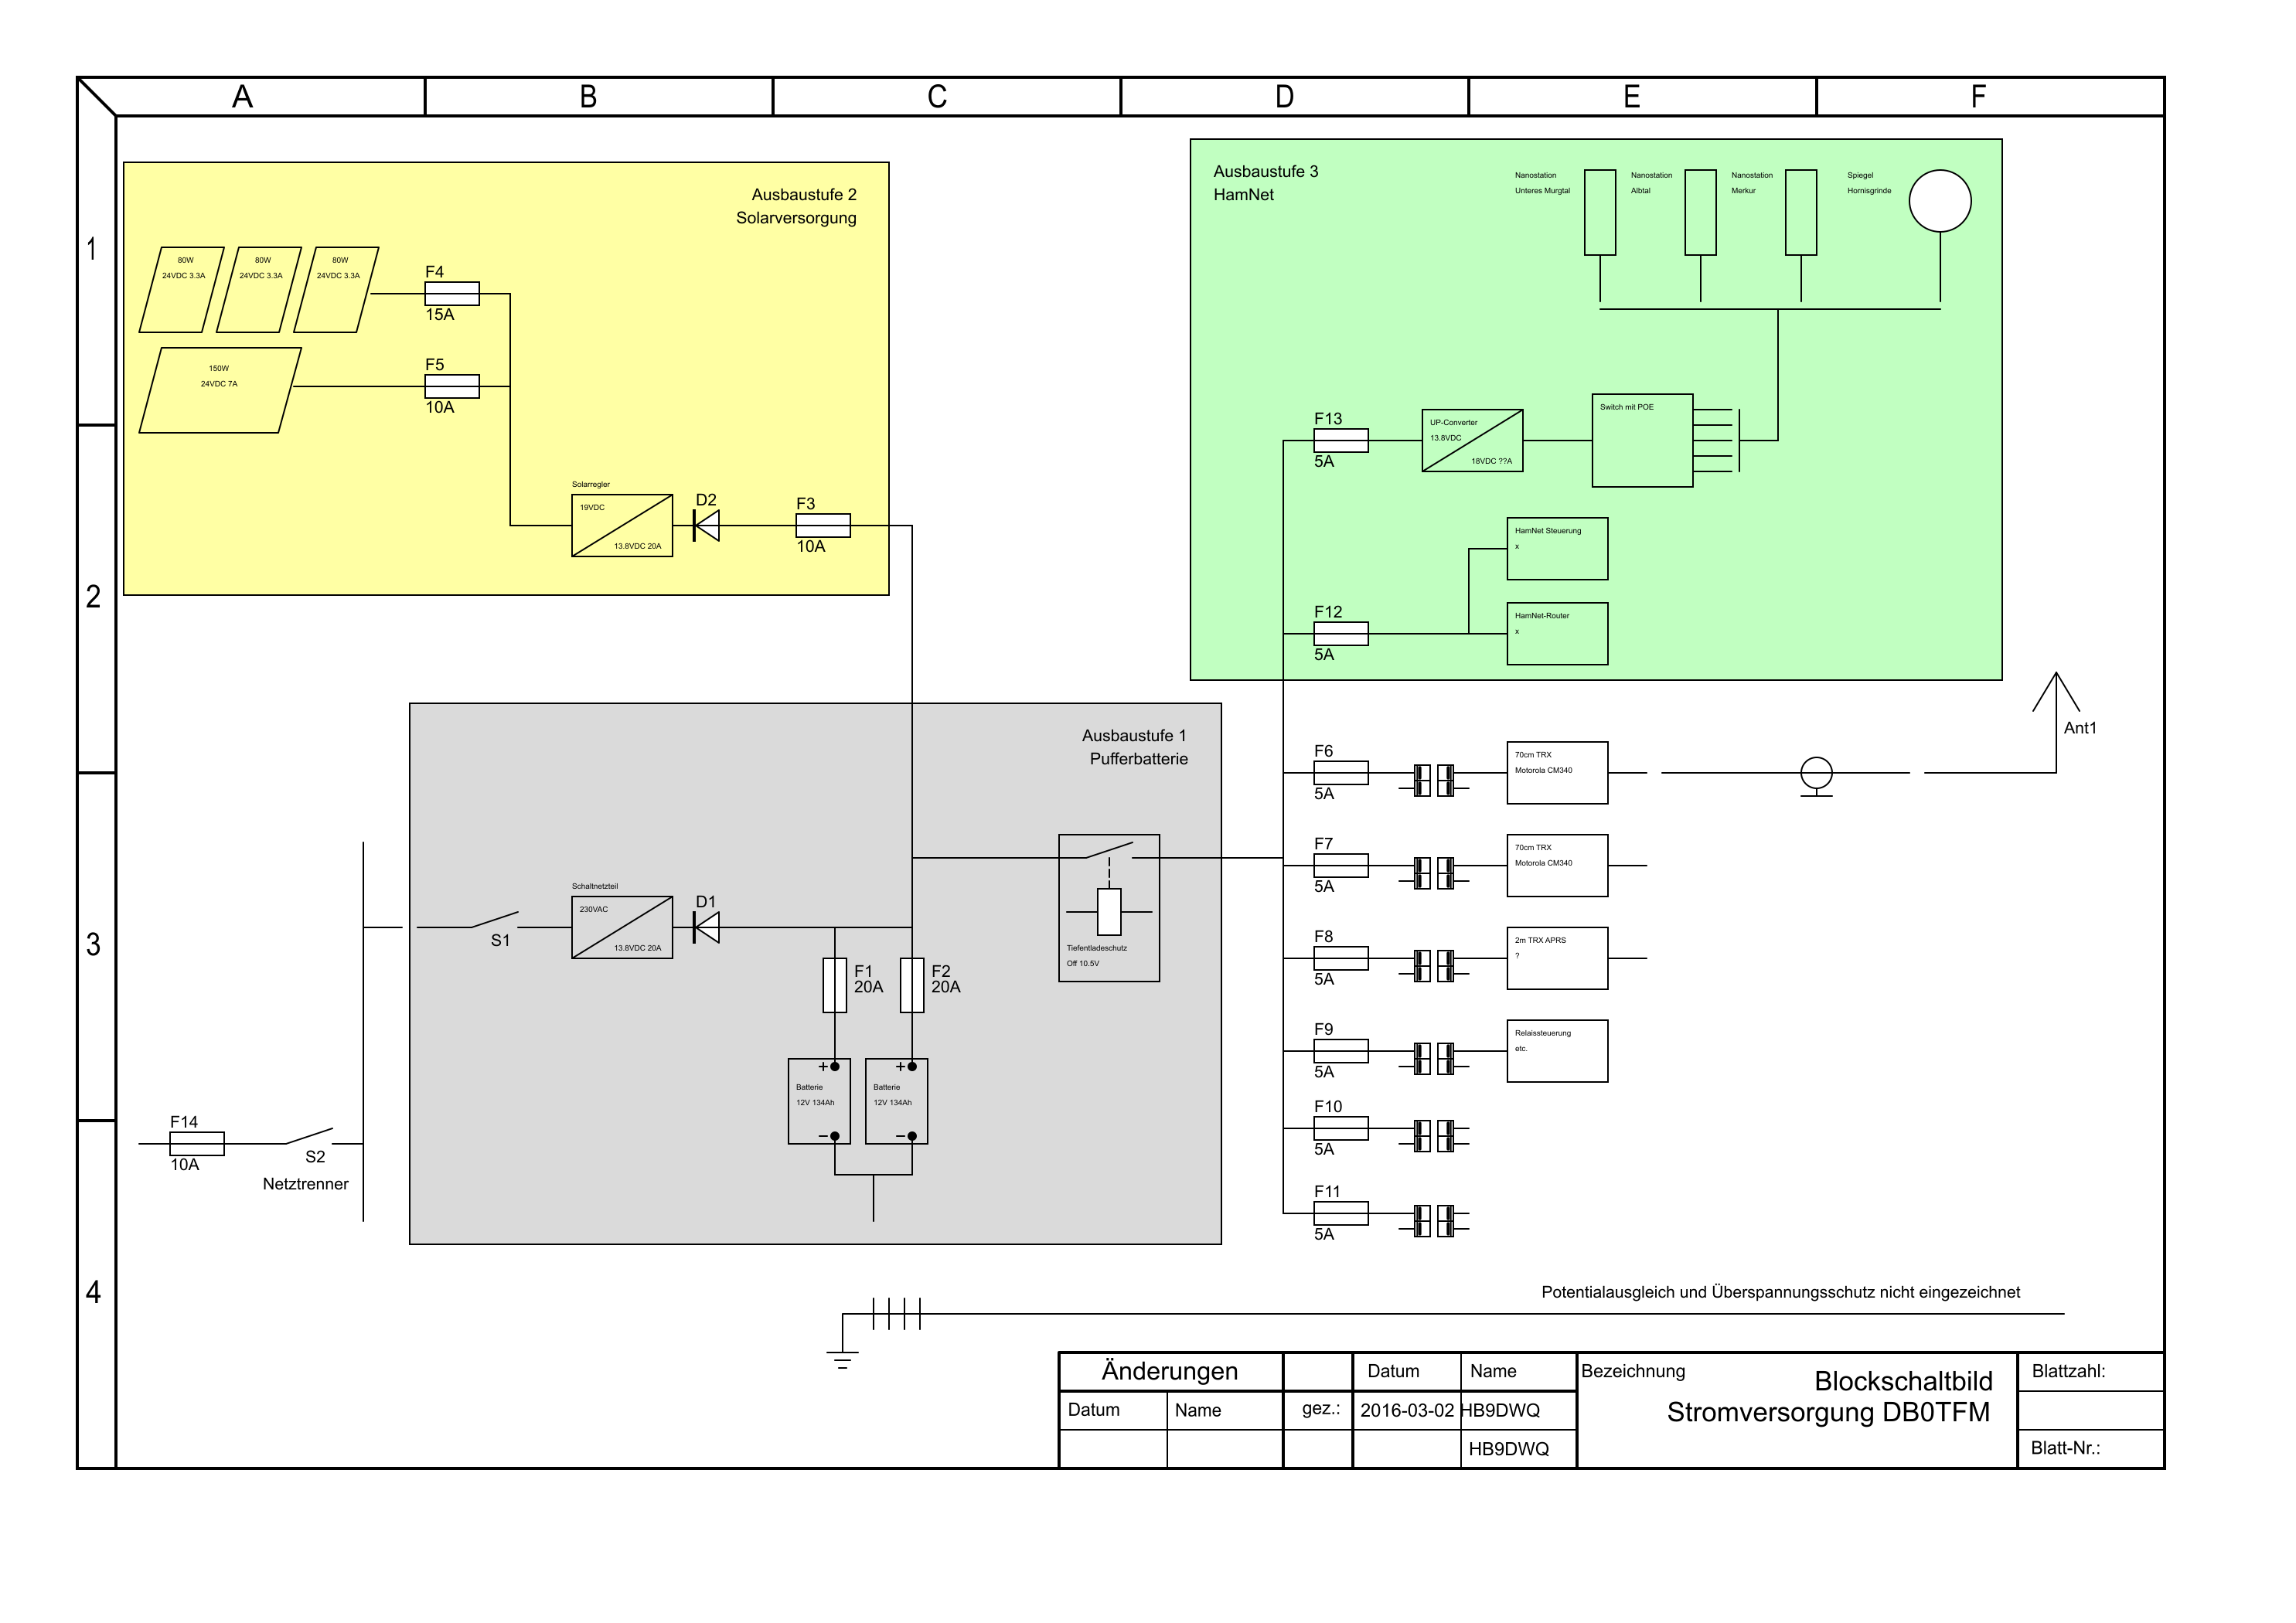
\includegraphics[height=\linewidth, angle=90]{Bilder/Blockschaltbild_Stromversorgung.png}

\section{Potentielle Linkstrecken}
\subsection{DB0OFG, Hornisgrinde}
Vorl\"aufig verworfen, Linkpartner bevorzugt andere Strecke.

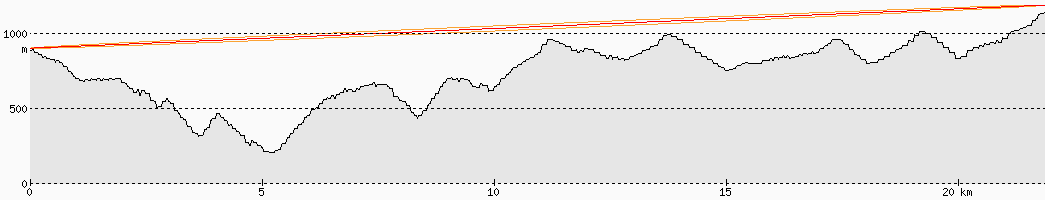
\includegraphics[width=\linewidth]{Bilder/Profil_DB0OFG.png}

\subsection{DB0SWF}
Linkpartner nicht erreicht.

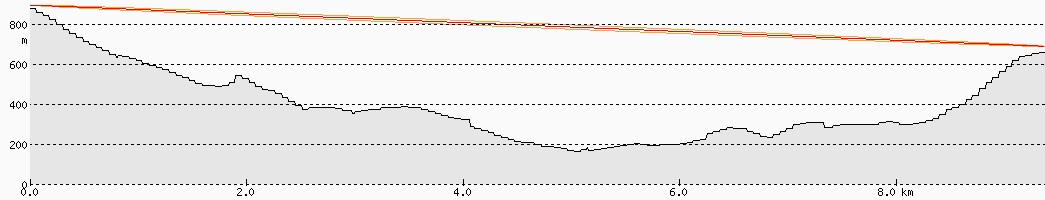
\includegraphics[width=\linewidth]{Bilder/Profil_DB0SWF}

\subsection{DL1FBE}
Internet-Bridge, nicht dringend

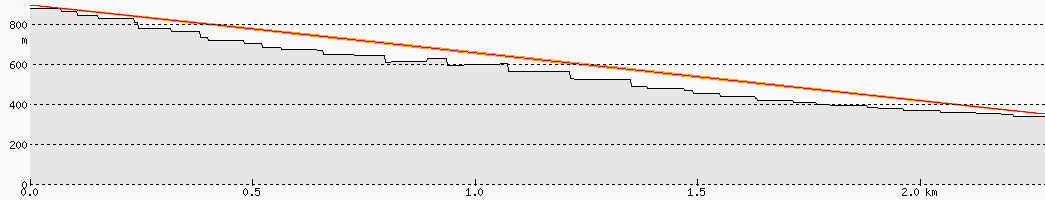
\includegraphics[width=\linewidth]{Bilder/Profil_DL1FBE}

\subsection{DL5IN}
Zwei Standorte, Linkstrecke zugesagt falls m\"oglich

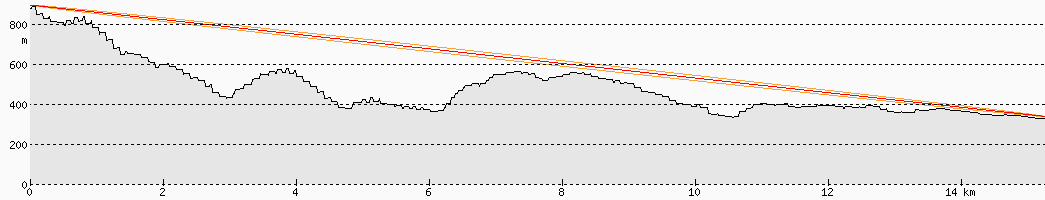
\includegraphics[width=\linewidth]{Bilder/Profil_DL5IN_48_877408_8_507792.png}

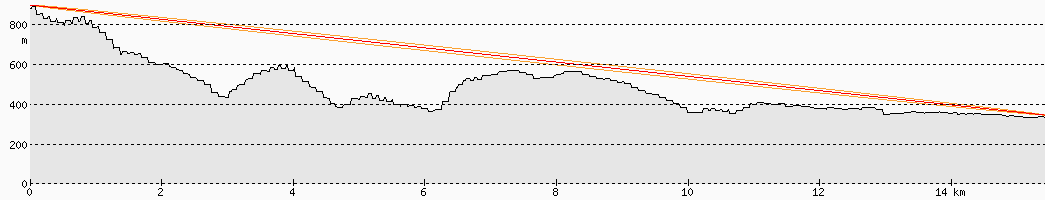
\includegraphics[width=\linewidth]{Bilder/Profil_DL5IN_48_877956_8_511058.png}

\subsection{Endg\"ultig verworfene Linkstrecken}
\begin{description}
    \item[DM0B] Existiert nicht mehr
    \item[DB0UX] Bessere Optionen mit dem gleichen Linkpartner verf\"ugbar
    \item[DB0UZ] Kann keine weiteren Antennen aufnehmen
    \item[DB0UKA] Keine Sichtverbindung
    \item[DB0HM] Keine Sichtverbindung
\end{description}
\end{document}
